%! Author = mishi9
%! Date = 24-09-20

A software defined radio (SDR) ADALM-PLUTO, will be used to transmit and receive radio waves, between 325 and 3800 MHz.
Patch antennas will be etched and submerged in the mixture.
On the end of those antenna PCBs there will be sockets for attaching cables that run from the SDR to the antennas.

\begin{center}
    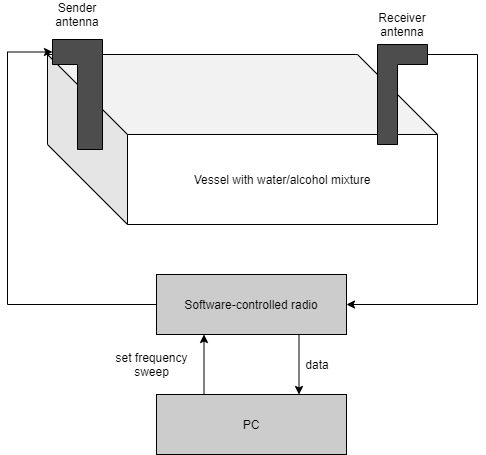
\includegraphics[scale=0.35]{sensor_system.png}
\end{center}

A program will be made to transmit and receive a frequency sweep of radio waves.
The impedance formula is:


\begin{align}
    Z(\omega) = \frac{E_o \sin(\omega t)}{I_o \sin(\omega t + \phi)} \\
    Z = \sqrt(\frac{\mu}{\epsilon})
\end{align}

Where Z is impedance, $E_o$ is excitement amplitude,
$\omega$ is radial frequency,
$I_o$ is response amplitude,
$\phi$ is phase,
$\epsilon$ and $\mu$ are the permittivity and permeability of the substance respectively.
Water and alcohol have insignificant difference in the permeability, therefore all of the difference in the impedance is a result of the different permittivities.
Threfore the ratio of the mixture's dielectroc constant to the control sample can be found out.
The formula of a mixture's dielectric constant is:

\begin{align}
    \epsilon_m = \epsilon_2 + \left( \epsilon_1 - \epsilon_2 \right) \sigma_1
\end{align}
where $\epsilon_m$ is the mixture's dielectric constant, $\epsilon_1$ and $\epsilon_2$ are the dielectric constants of the mixed elements and $\sigma_1$ is the concentration of the first solvent in the mixture.
This formula can be rearranged to get that
\begin{align}
    \sigma_1 = \frac{\epsilon_2 - \epsilon_m}{\epsilon_2 - \epsilon_1}
\end{align}
If we know the dielectric constant of the mixture, and the separate constants for pure water and pure ethyl alcohol, we can determine the ratio of water-to-alcohol in the mixture.